\section{Regression and variable selection}
\begin{slide}\slidetitle{Regression and variable selection}
\tableofcontents[sectionstyle=show/hide,subsectionstyle=show/shaded/hide]

\end{slide}
\subsection{Regression}\begin{slide}\slidetitle{Regression}

Large fraction of statistical analyses dealing with representation of dependences between several 
variables, rather than marginal distribution of each variable

\end{slide}\begin{slide}\slidetitle{Pine processionary caterpillars}

\begin{columns}
\column{.45\textwidth}
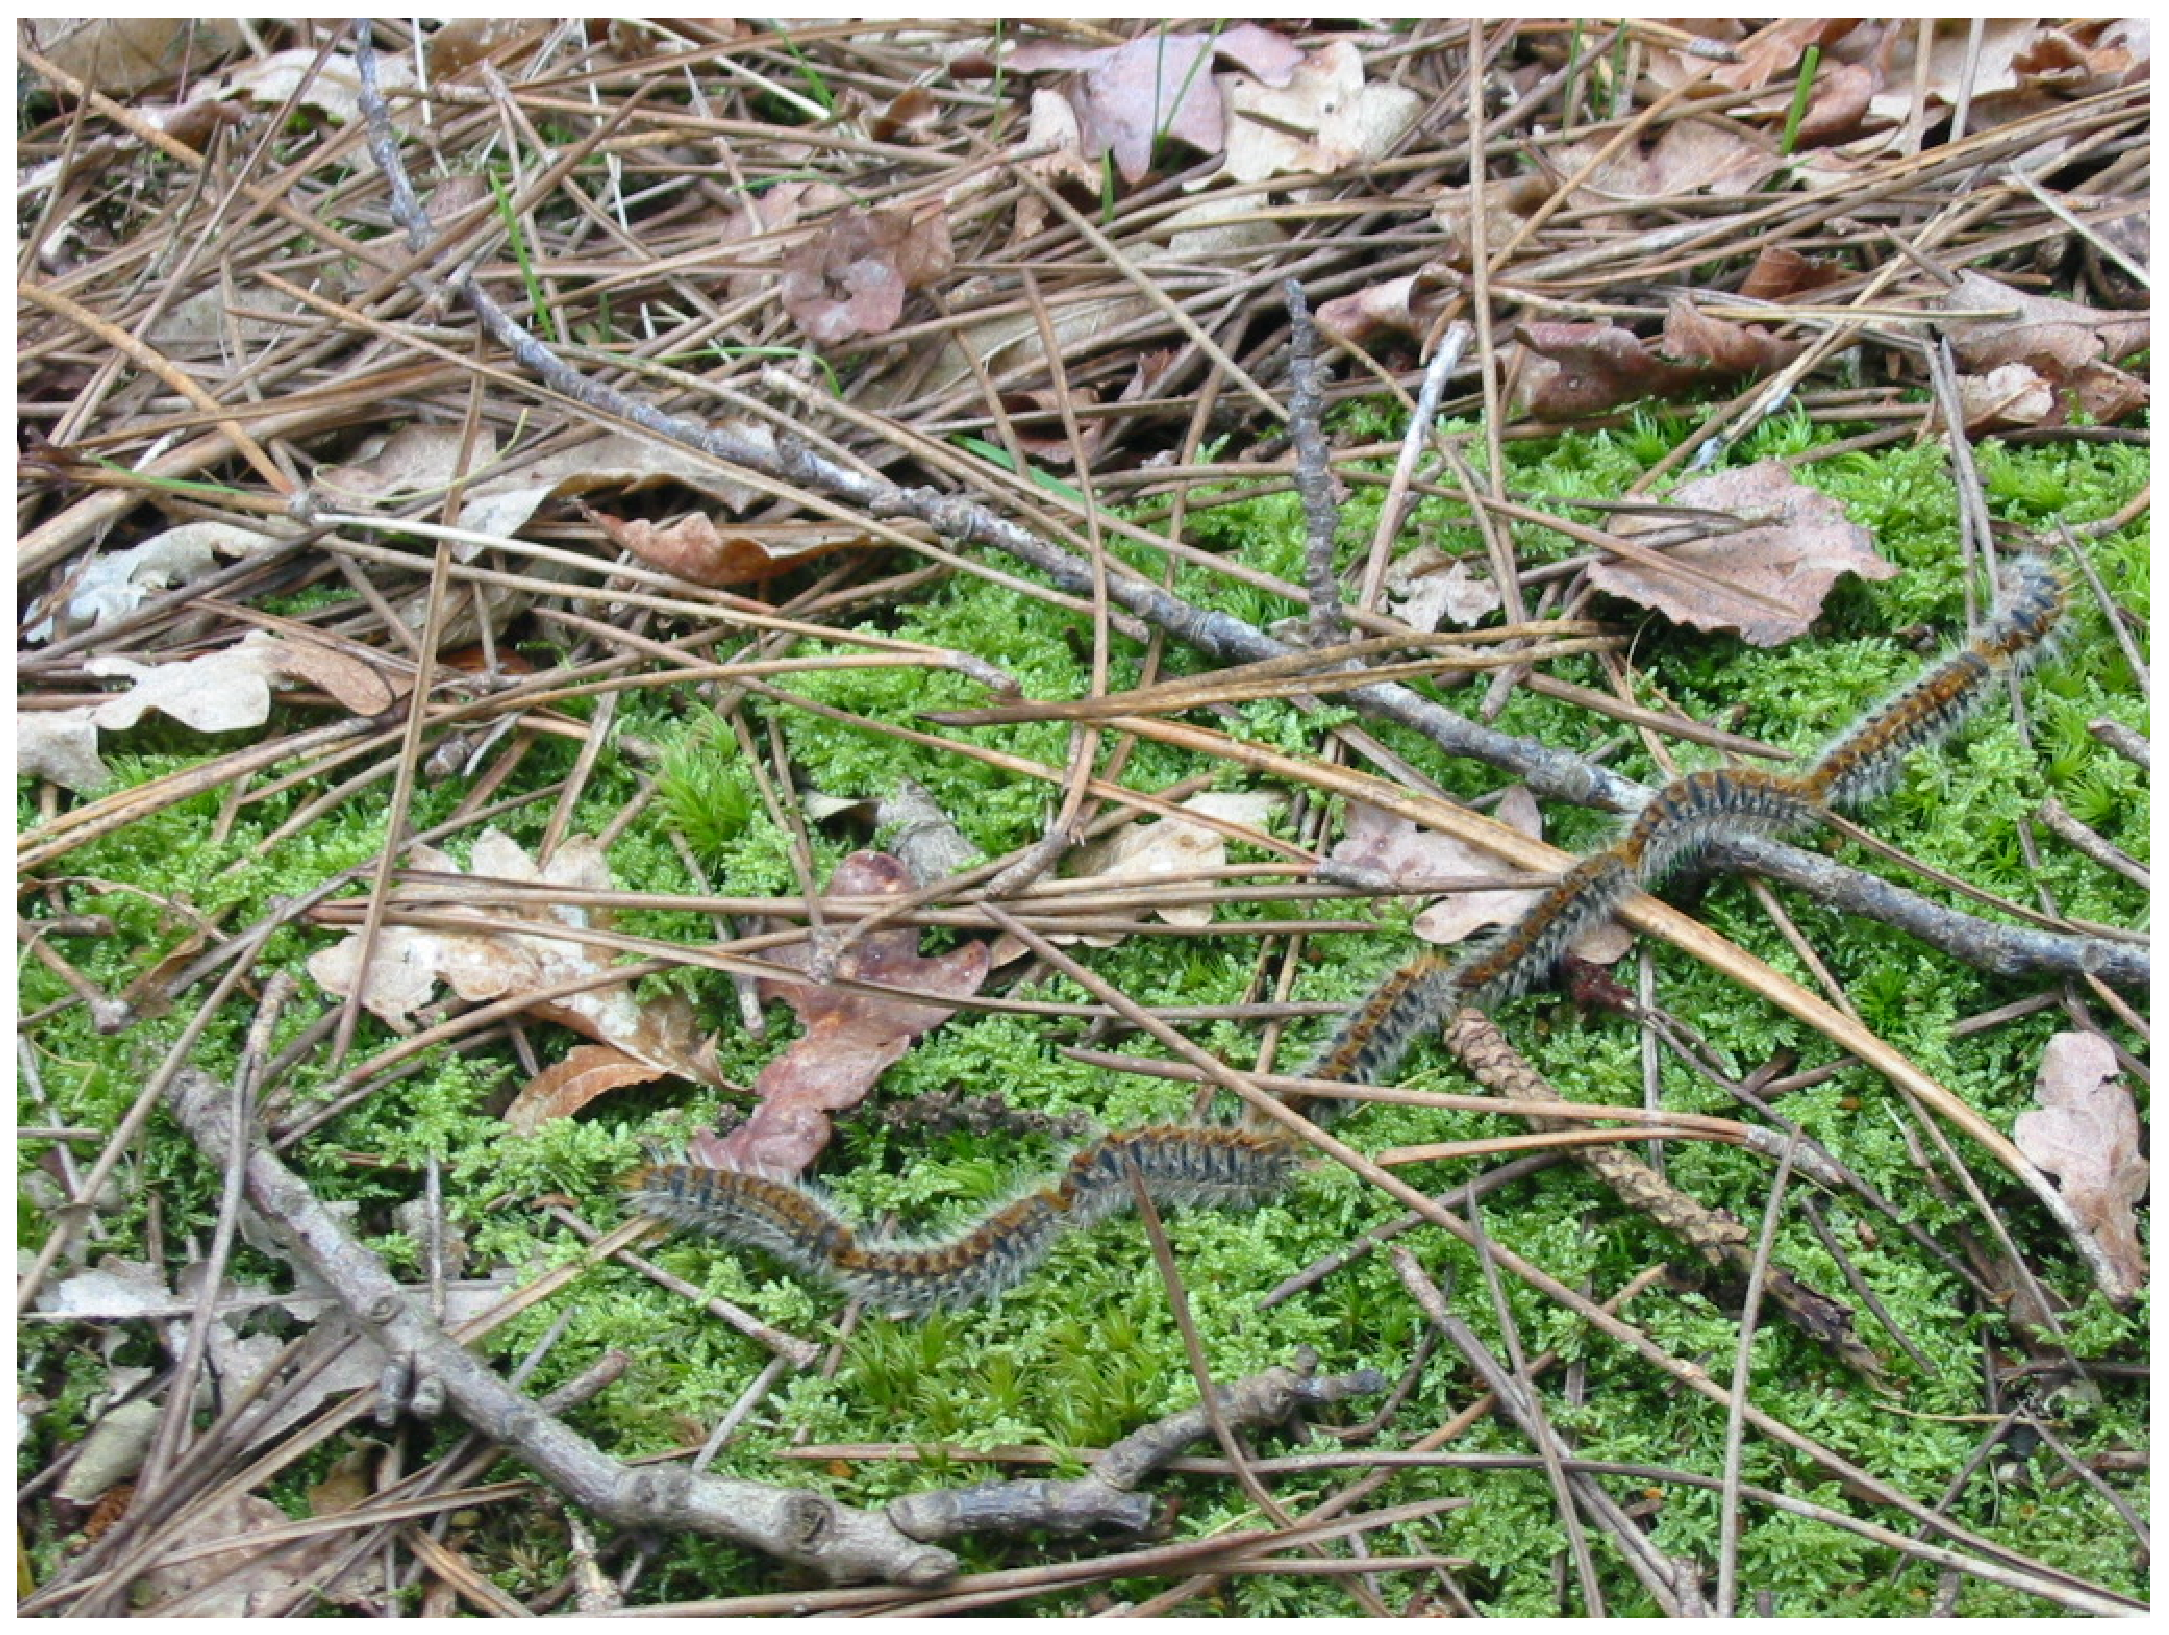
\includegraphics[width=5cm]{figures/caterpibreizh.eps}
\pause
\column{.45\textwidth}
\only<2>{Pine processionary caterpillar colony size influenced by
\tiny
\begin{itemize}
\item[] $x_1$ altitude
\item[] $x_2$ slope (in degrees)
\item[] $x_3$ number of pines in the area
\item[] $x_4$ height of the central tree
\item[] $x_5$ diameter of the central tree
\item[] $x_6$ index of the settlement density
\item[] $x_7$ orientation of the area (from $1$ [southbound] to $2$)
\item[] $x_8$ height of the dominant tree
\item[] $x_9$ number of vegetation strata
\item[] $x_{10}$ mix settlement index (from $1$ if not mixed to $2$ if mixed)
\end{itemize}
\normalsize}
\only<3>{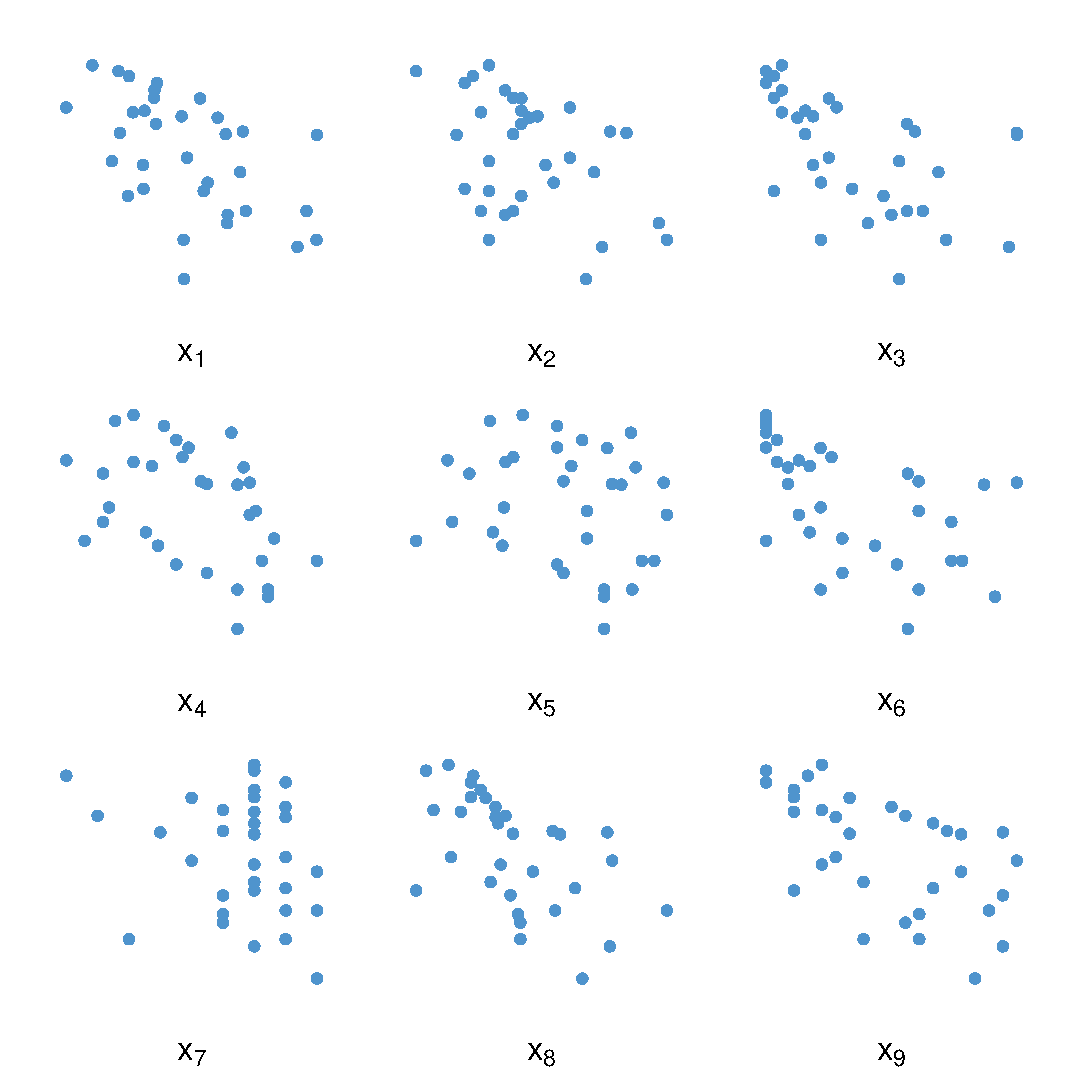
\includegraphics[width=5cm]{figures/processimpl.eps}}
\end{columns}

\end{slide}\begin{slide}\slidetitle{Goal of a regression model}

From a statistical point of view, find a proper representation
of the distribution, $f(y|\theta,x)$, of an observable variable $y$ 
given a vector of observables $x$, based on a sample of $(x,y)_i$'s. 

\end{slide}\begin{slide}\slidetitle{Linear regression}

Linear regression: one of the most widespread tools of Statistics for analysing (linear) influence 
of some variables or some factors on others

\vs\pause
\begin{block}{Aim}{\centerline{\BurntOrange{To uncover explanatory and predictive patterns}}}\end{block}

\end{slide}\begin{slide}\slidetitle{Regressors and response}

Variable of primary interest, $y$, called the \textit{response} or the \textit{outcome} variable
[assumed here to be continuous]

\begin{flushright}E.g., number of Pine processionary caterpillar colonies\end{flushright}

\pause
Covariates $x=(x_1,\ldots,x_k)$ called \textit{explanatory variables} [may be discrete, 
continuous or both]

\pause
\vs Distribution of $y$ given $x$ typically studied in the context of a set of \textit{units} or
experimental \textit{subjects},  $i=1,\ldots,n$, for instance patients in an hospital ward,
on which both $y_i$ and $x_{i1},\ldots,x_{ik}$ are measured.

\end{slide}\begin{slide}\slidetitle{Regressors and response cont'd}

Dataset made of the conjunction of the vector of outcomes
$$
y=\left(y_1,\ldots,y_n\right)
$$ 
\pause
and of the $n\times (k+1)$ matrix of explanatory variables
$$
X=\left[\begin{array}{ccccc}
 1      & x_{11} & x_{12} & \ldots & x_{1k} \\
 1      & x_{21} & x_{22} & \ldots & x_{2k} \\
 1      & x_{31} & x_{32} & \ldots & x_{3k} \\
 \vdots & \vdots & \vdots & \vdots & \vdots \\
 1      & x_{n1} & x_{n2} & \ldots & x_{nk}
\end{array}\right]
$$

\end{slide}\subsection{Linear models}
\begin{slide}\slidetitle{Linear models}

\textit{Ordinary normal linear regression} model such that
$$
y|\beta,\sigma^2,X\sim\mathscr{N}_n(X\beta,\sigma^2I_n)
$$
\pause
and thus
\begin{eqnarray*}
\mathbb{E}[y_i|\beta,X]    &=& \beta_0+\beta_1x_{i1}+\ldots+\beta_kx_{ik}\\
\mathbb{V}(y_i|\sigma^2,X) &=& \sigma^2
\end{eqnarray*}

\end{slide}\begin{slide}\slidetitle{Categorical variables}

\begin{itemize}
\item[{\Large $\lightning$}]
There \BrickRed{is} a difference between finite valued regressors like $x_7$ in {\sf caterpillar} 
\Brown{[orientation of the area]} and
{\em categorical} variables (or {\em factors}), which are also taking a finite number of values
but whose range has no numerical meaning.
\end{itemize}

\pause
\begin{example}
If $x$ is the socio-professional category of an employee, this variable ranges from $1$ to $9$ 
for a rough grid of socio-professional activities, and from $1$ to $89$ on a finer grid. 

\BurntOrange{\centerline{The numerical values are not comparable}}
\end{example}

\end{slide}\begin{slide}\slidetitle{Categorical variables (cont'd)}

Makes little sense to involve $x$ directly in the regression: replace the single regressor $x$ [in
$\{1,\ldots,m\}$, say] with $m$ indicator (or {\em dummy}) variables 
$$
x_1=\mathbb{I}_1(x), \ldots, x_m=\mathbb{I}_m(x)
$$

\pause
\begin{block}{\BrickRed{Convention}}
Use of a different constant $\beta_i$ for each class categorical variable value:
$$
\mathbb{E}[y_i|\beta,X] = \ldots + \beta_1\mathbb{I}_1(x)+\ldots+\beta_m\mathbb{I}_m(x)+\ldots
$$
\end{block}

\end{slide}\begin{slide}
\slidetitle{Identifiability}

Identifiability issue: For dummy variables, sum of the indicators equal to one.


\begin{block}{Convention}
Assume that $X$ is of full rank:
$$\BrickRed{
\mbox{rank}(X)=k+1
}$$
[$X$ is of full rank if and only if $X^\tee X$ is invertible]
\end{block}

\pause
\begin{flushright} E.g., for dummy variables, this means eliminating one class \end{flushright}

\end{slide}\begin{slide}
\slidetitle{Likelihood function \&\ estimator}

The likelihood of the \textit{ordinary normal linear model} is
$$
\ell\left(\beta,\sigma^2|y,X\right)=\left(2\pi\sigma^2\right)^{-n/2}\,
\exp\left[-\frac{1}{2\sigma^2}(y-X\beta)^\tee (y-X\beta)\right]
$$

\pause\vs The MLE of $\beta$ is solution of the least squares minimisation problem
\small
$$
\min_\beta\, (y-X\beta)^\tee (y-X\beta) = \min_\beta
\,\sum_{i=1}^n\left(y_i-\beta_0-\beta_1x_{i1}-\ldots-\beta_kx_{ik}\right)^2\,,
$$
\normalsize
namely
$$\BrickRed{
\hat\beta=(X^\tee X)^{-1}X^\tee y
}$$

\end{slide}\begin{slide}
\slidetitle{Least square estimator}
\begin{itemize}
\item $\hat\beta$ is an unbiased estimator of $\beta$.

\item $\mathbb{V}(\hat\beta|\sigma^2,X)=\sigma^2(X^\tee X)^{-1}$

\item $\hat\beta$ is the {\em best} linear unbiased estimator of $\beta$: 
for all $a\in\mathbb{R}^{k+1}$, 
$$
\mathbb{V}(a^\tee\hat\beta|\sigma^2,X)\leq\mathbb{V} (a^\tee\tilde\beta|\sigma^2,X)
$$
for any unbiased linear estimator $\tilde\beta$ of $\beta$.

\item Unbiased estimator of $\sigma^2$
$$
\hat\sigma^2=\frac{1}{n-k-1}(y-X\hat\beta)^\tee (y-X\hat\beta)=\frac{s^2}{n-k-1},
$$
\end{itemize}

\end{slide}
\begin{frame}[fragile]
\frametitle{Pine processionary caterpillars}

\footnotesize
\begin{verbatim}
Residuals:        Min       1Q     Median     3Q        Max
                -1.6989  -0.2731   -0.0003  0.3246     1.7305
Coefficients:
             Estimate Std. Error t value Pr(>|t|)
intercept   10.998412   3.060272   3.594  0.00161 **
XV1         -0.004431   0.001557  -2.846  0.00939 **
XV2         -0.053830   0.021900  -2.458  0.02232 * 
XV3          0.067939   0.099472   0.683  0.50174
XV4         -1.293636   0.563811  -2.294  0.03168 *
XV5          0.231637   0.104378   2.219  0.03709 *
XV6         -0.356800   1.566464  -0.228  0.82193
XV7         -0.237469   1.006006  -0.236  0.81558
XV8          0.181060   0.236724   0.765  0.45248
XV9         -1.285316   0.864847  -1.486  0.15142
XV10        -0.433106   0.734869  -0.589  0.56162
---
Signif. codes:  
0 `***' 0.001 `**' 0.01 `*' 0.05 `.' 0.1 ` ' 1
\end{verbatim}
\normalsize

\end{frame}
\subsection{Zellner's informative $G$-prior}
%\newcommand\by{\mathbf{y}}
\begin{slide}\slidetitle{Conjugate priors}

If [conditional prior] 
$$
\beta|\sigma^2,X\sim\mathscr{N}_{k+1}(\tilde\beta,\sigma^2M^{-1})\,,
$$
where $M$ $(k+1,k+1)$ positive definite symmetric matrix, and 
$$
\sigma^2|X\sim \mathscr{IG}(a,b),\qquad a,b>0,
$$
\pause then
\small
$$
\beta|\sigma^2,\by,X\sim
\mathscr{N}_{k+1}\left((M+X^\tee X)^{-1}
\{(X^\tee X)\hat\beta+M\tilde\beta\},\sigma^2(M+X^\tee X)^{-1}\right)
$$
and 
$$
\sigma^2|\by,X\sim
\mathscr{IG}\left(\frac{n}{2}+a,b+\frac{s^2}{2}+\frac{(\tilde\beta-\hat\beta)^\tee
\left(M^{-1}+(X^\tee X)^{-1}\right)^{-1}(\tilde\beta-\hat\beta)}{2}\right)
$$
\normalsize

\end{slide}
\begin{slide}\slidetitle{Experimenter dilemma}

Problem of the choice of $M$ or of $c$ if $M=I_{k+1}/c$

\pause
\begin{example}[Processionary caterpillar]
No precise prior information about $\tilde\beta$, $M$, $a$ and $b$. Take
$a=2.1$ and $b=2$, i.e.~prior mean and prior variance of $\sigma^2$ equal to
$1.82$ and $33.06$, and $\tilde\beta=0_{k+1}$.

\pause
Lasting influence of $c$: 
\small
\begin{center}\begin{tabular}{r r r r}
        $c$ &  $\ \mathbb{E}^\pi(\sigma^2|\by,X)$ & $\ \mathbb{E}^\pi(\beta_0|\by,X)$ & $\ \mathbb{V}^\pi(\beta_0|\by,X)$ \\
    \hline
   .1 &  1.0044 &  0.1251 & 0.0988 \\
   1   &  0.8541 &  0.9031 & 0.7733 \\
  10   &  0.6976 &  4.7299 & 3.8991 \\
 100   &  0.5746 &  9.6626 & 6.8355 \\
1000   &  0.5470 & 10.8476 & 7.3419
\end{tabular}\end{center}
\normalsize
\end{example}

\end{slide}
\begin{slide}\slidetitle{Zellner's informative $G$-prior}

\begin{block}{Constraint}
Allow the experimenter to 
introduce information about the location parameter of the regression 
while bypassing the most difficult aspects of the prior specification, 
namely the derivation of the prior correlation structure. 
\end{block}

\pause
\vs Zellner's prior corresponds to
\begin{eqnarray*}\BrickRed{
\beta|\sigma^2,X &\sim& \mathscr{N}_{k+1}(\tilde\beta,c\sigma^2(X^\tee X)^{-1})\\
\sigma^2 &\sim& \pi(\sigma^2|X)\propto\sigma^{-2}\,.
}\end{eqnarray*}
\emfarite{Special conjugate}

\end{slide}\begin{slide}
\slidetitle{Prior selection}

Experimental prior determination restricted to the choices of $\tilde\beta$ and of the constant $c$. 

\medskip\begin{block}{Note} 
$c$ can be interpreted as a measure of the amount of information available in the prior 
relative to the sample. For instance, setting $1/c=0.5$ gives the prior the same weight 
as 50\% of the sample.
\end{block}

\pause
\begin{itemize}
\item[{\Large $\lightning$}]
There still \BrickRed{is} a lasting influence of the factor $c$
\end{itemize}

\end{slide}\begin{slide}
\slidetitle{Posterior structure}
With this prior model, the posterior simplifies into
\small
\begin{eqnarray*}
\pi(\beta,\sigma^2|y,X) & \propto & f(y|\beta,\sigma^2,X)\pi(\beta,\sigma^2|X) \\
&\propto& \left(\sigma^2\right)^{-(n/2+1)}\exp\left[-\frac{1}{2\sigma^2}(y-X\hat\beta)^\tee 
   (y-X\hat\beta)\right.\\
&&\quad \left.-\frac{1}{2\sigma^2}(\beta-\hat\beta)^\tee X^\tee X(\beta-\hat\beta)\right]
	\left(\sigma^2\right)^{-k/2}\\
&&\quad\times \exp\left[-\frac{1}{2c\sigma^2}(\beta-\tilde\beta)X^\tee X(\beta-\tilde\beta)\right]\,,
\end{eqnarray*}
\normalsize
because $X^\tee X$ used in both prior and likelihood 
\emfarite{$G$-prior trick}

\end{slide}\begin{slide}
\slidetitle{Posterior structure (cont'd)}
Therefore,
\begin{eqnarray*}
\beta|\sigma^2,y,X&\sim&\mathscr{N}_{k+1}\left(\frac{c}{c+1}(\tilde\beta/c+\hat\beta),
\frac{\sigma^2c}{c+1}(X^\tee X)^{-1}\right)\\
\sigma^2|y,X&\sim&\mathcal{IG}\left(\frac{n}{2},\frac{s^2}{2}+\frac{1}{2(c+1)}
(\tilde\beta-\hat\beta)^\tee X^\tee X(\tilde\beta-\hat\beta)\right)
\end{eqnarray*}
and
\small
\begin{eqnarray*}
\beta|y,X &\sim& \mathscr{T}_{k+1}\left(n,\frac{c}{c+1}\left(\frac{\tilde\beta}{c}+\hat\beta\right),\right. \\
&& \left.\frac{c(s^2+(\tilde\beta-\hat\beta)^\tee X^\tee 
X(\tilde\beta-\hat\beta)/(c+1))}{n(c+1)}(X^\tee X)^{-1}\right).
\end{eqnarray*}
\normalsize

\end{slide}\begin{slide}\slidetitle{Bayes estimator}

The Bayes estimators of $\beta$ and $\sigma^2$ are given by
$$
\mathbb{E}^\pi[\beta|y,X]=\frac{1}{c+1}(\tilde\beta+c\hat\beta)
$$
and
$$
\mathbb{E}^\pi[\sigma^2|y,X]=\frac{s^2+(\tilde\beta-\hat\beta)^\tee X^\tee X(\tilde\beta-\hat\beta)/(c+1)}{n-2}\,.
$$ 

\medskip\pause
{\bf Note:}
Only when $c$ goes to infinity does the influence of the prior vanish!

\end{slide}\begin{slide}
\slidetitle{Pine processionary caterpillars}

\only<1>{\begin{center}
\begin{tabular}{c|r r}
$\beta_i$ & $\ \mathbb{E}^\pi(\beta_i|\by,X)\ $ & $\ \mathbb{V}^\pi(\beta_i|\by,X)$ \\
 \hline $\beta_0$ & 10.8895 & 6.4094 \\
 $\beta_1$ & -0.0044 & 2e-06 \\
 $\beta_2$ & -0.0533 & 0.0003 \\
 $\beta_3$ &  0.0673 & 0.0068 \\
 $\beta_4$ & -1.2808 & 0.2175 \\
 $\beta_5$ &  0.2293 & 0.0075 \\
 $\beta_6$ & -0.3532 & 1.6793 \\
 $\beta_7$ & -0.2351 & 0.6926 \\
 $\beta_8$ &  0.1793 & 0.0383 \\
 $\beta_9$ & -1.2726 & 0.5119 \\
 $\beta_{10}$ & -0.4288 & 0.3696
\end{tabular}

		$c=100$
\end{center}}

\end{slide}\begin{slide}
\slidetitle{Pine processionary caterpillars (2)}
\only<1>{
\begin{center}
\begin{tabular}{c|r r}
$\beta_i$ & $\ \mathbb{E}^\pi(\beta_i|\by,X)\ $ & $\ \mathbb{V}^\pi(\beta_i|\by,X)$ \\
 \hline $\beta_0$ & 10.9874 & 6.2604 \\
 $\beta_1$ & -0.0044 & 2e-06 \\
 $\beta_2$ & -0.0538 & 0.0003 \\
 $\beta_3$ &  0.0679 & 0.0066 \\
 $\beta_4$ & -1.2923 & 0.2125 \\
 $\beta_5$ &  0.2314 & 0.0073 \\
 $\beta_6$ & -0.3564 & 1.6403 \\
 $\beta_7$ & -0.2372 & 0.6765 \\
 $\beta_8$ &  0.1809 & 0.0375 \\
 $\beta_9$ & -1.2840 & 0.5100 \\
 $\beta_{10}$ & -0.4327 & 0.3670
\end{tabular}

		$c=1,000$
\end{center}}

\end{slide}\begin{slide}\slidetitle{Conjugacy}

Moreover,
\small
$$
\mathbb{V}^\pi[\beta|y,X]=\frac{c(s^2+(\tilde\beta-\hat\beta)^\tee 
X^\tee X(\tilde\beta-\hat\beta)/(c+1))}{n(c+1)}(X^\tee X)^{-1}\,.
$$
\normalsize

\pause
\BurntOrange{{\bf Convenient tool for translating prior information on 
$\beta$:}} For instance, if $c=1$, this is equivalent 
to putting the same weight on the prior information 
and on the sample:
$$
\mathbb{E}^\pi(\beta|y,X)=\left(\frac{\tilde\beta+\hat\beta}{2}\right)\,
$$
average between prior mean and maximum likelihood estimator.

\pause
If, instead, $c=100$, the prior gets a weight of 1\% of the sample. 

\end{slide}\begin{slide}\slidetitle{Predictive}

Prediction of $m\ge 1$ future observations from units in which the explanatory variables 
$\tilde X$---but not the outcome variable 
$$
\tilde y \sim \mathcal{N}_m(\tilde X\beta, \sigma^2I_m)
$$
---have been observed 

\pause
\vs {\em Predictive distribution} on $\tilde y$ defined as marginal of the joint posterior 
distribution on $(\tilde y,\beta,\sigma^2)$. Can be computed analytically by
$$
\int \pi(\tilde y|\sigma^2,y,X,\tilde X) \pi(\sigma^2|y,X,\tilde X)\,\text{d}\sigma^2\,. 
$$

\end{slide}\begin{slide}\slidetitle{Gaussian predictive}
Conditional on $\sigma^2$, the future vector of observations has a Gaussian distribution with
\small
\begin{eqnarray*}
\mathbb{E}^\pi[\tilde y|\sigma^2,y,X,\tilde X] 
& = & \mathbb{E}^\pi[\mathbb{E}^\pi(\tilde y|\beta,\sigma^2,y,X,\tilde X)|\sigma^2,y,X,\tilde X] \\
                                  & = & \mathbb{E}^\pi[\tilde X\beta|\sigma^2,y,X,\tilde X] \\
                                  & = & \tilde X\frac{\tilde\beta+c\hat\beta}{c+1}
\end{eqnarray*}
\normalsize
independently of $\sigma^2$. \pause Similarly,
\small
\begin{eqnarray*}
\mathbb{V}^\pi(\tilde y|\sigma^2,y,X,\tilde X) 
& = & \mathbb{E}^\pi[\mathbb{V}(\tilde y|\beta,\sigma^2,y,X,\tilde X)|\sigma^2,y,X,\tilde X] \\
                  &&\quad +\mathbb{V}^\pi[\mathbb{E}^\pi(\tilde y|\beta,\sigma^2,y,X,\tilde X)|\sigma^2,y,X,\tilde X] \\
                  &=& \mathbb{E}^\pi[\sigma^2I_m|\sigma^2,y,X,\tilde X]+\mathbb{V}^\pi(\tilde X\beta|\sigma^2,y,X,\tilde X) \\
                  &=& \sigma^2\left(I_m+\frac{c}{c+1}\tilde X(X^\tee X)^{-1}\tilde X^\tee \right)
\end{eqnarray*}
\normalsize

\end{slide}\begin{slide}\slidetitle{Predictor}

A predictor under squared error loss is the posterior predictive mean
$$
\tilde X\frac{\tilde\beta+c\hat\beta}{c+1}\,,
$$

Representation quite intuitive, 
being the product of the matrix of explanatory variables 
$\tilde X$ by the Bayes estimate of $\beta$.

\end{slide}\begin{slide}\slidetitle{Credible regions}
Highest posterior density (HPD) regions on subvectors of the parameter $\beta$ derived 
from the marginal posterior distribution of $\beta$. \pause For a single parameter,
\small
\begin{eqnarray*}
\beta_i|y,X &\sim& \mathscr{T}_1\left(n,\frac{c}{c+1}\left(\frac{\tilde\beta_i}{c}
		+\hat\beta_i\right),\right. \\
            && \qquad \left.\frac{c(s^2+(\tilde\beta-\hat\beta)^\tee X^\tee X
		(\tilde\beta-\hat\beta)/(c+1))}{n(c+1)}\omega_{(i,i)}\right)\,,
\end{eqnarray*}
\normalsize
where $\omega_{(i,i)}$ is the $(i,i)$-th element of the matrix $(X^\tee X)^{-1}$. 

\end{slide}\begin{slide}\slidetitle{$T$ time}

If
$$
\tau=\frac{\tilde\beta+c\hat\beta}{c+1}$$
and
$$
K=\frac{c(s^2+(\tilde\beta-\hat\beta)^\tee X^\tee X(\tilde\beta-\hat\beta)/(c+1))}{n(c+1)}(X^\tee X)^{-1}
 =\left( \kappa_{(i,j)} \right)\,,
$$
the transform
$$
\mathfrak{T}_i = \frac{\beta_i-\tau_i}{\sqrt{\kappa_{(i,i)}}}
$$
has a standard $t$ distribution with $n$ degrees of freedom. 

\end{slide}\begin{slide}\slidetitle{$T$ HPD}

A $1-\alpha$ HPD 
interval on $\beta_i$ is thus given by
$$
\left[\tau_i-\sqrt{\kappa_{(i,i)}}F_{n}^{-1}(1-\alpha/2),\tau_i+\sqrt{\kappa_{(i,i)}}F_{n}^{-1}(1-\alpha/2)\right].
$$

\end{slide}\begin{frame}
\frametitle{Pine processionary caterpillars}

\begin{center}
\begin{tabular}{c|c}
 $\beta_i\ $ & HPD interval\\
 \hline $\beta_0$ & $[5.7435,16.2533]$ \\
 $\beta_1$ & \ $[-0.0071,-0.0018]$ \\
 $\beta_2$ & \ $[-0.0914,-0.0162]$ \\
 $\beta_3$ & \ $[-0.1029,0.2387]$ \\
 $\beta_4$ & \ $[-2.2618,-0.3255]$ \\
 $\beta_5$ & \ $[0.0524,0.4109]$ \\
 $\beta_6$ & \ $[-3.0466,2.3330]$ \\
 $\beta_7$ & \ $[-1.9649,1.4900]$ \\
 $\beta_8$ & \ $[-0.2254,0.5875]$ \\
 $\beta_9$ & \ $[-2.7704,0.1997]$ \\
 $\beta_{10}$ & \ $[-1.6950,0.8288]$
\end{tabular}
\end{center}
$$
c=100
$$
\end{frame}\begin{slide}\slidetitle{$T$ marginal}
\MidnightBlue{{\bf Marginal distribution of $y$ is multivariate $t$ distribution}}

\vs\small
{\bf Proof.} Since $\beta|\sigma^2,X\sim\mathscr{N}_{k+1}(\tilde\beta,c\sigma^2(X^\tee X)^{-1})$, 
$$
X\beta|\sigma^2,X\sim\mathscr{N}(X\tilde\beta,c\sigma^2X(X^\tee X)^{-1}X^\tee )\,,
$$
which implies that
$$
y|\sigma^2,X\sim\mathscr{N}_n(X\tilde\beta,\sigma^2(I_n+cX(X^\tee X)^{-1}X^\tee )).
$$
Integrating in $\sigma^2$ yields
\begin{eqnarray*}
f(y|X) & = & (c+1)^{-(k+1)/2}\pi^{-n/2}\Gamma(n/2) \\
       &   &\times \left[y^\tee y-\frac{c}{c+1}y^\tee X(X^\tee X)^{-1}X^\tee y-\frac{1}{c+1}\tilde\beta^\tee 
		X^\tee X\tilde\beta\right]^{-n/2}.
\end{eqnarray*}
\normalsize

\end{slide}\begin{slide}\slidetitle{Point null hypothesis}

If a null hypothesis is $H_0:R\beta=r$, the model under $H_0$ can be rewritten as
$$
y|\beta^0,\sigma^2,X_0\stackrel{H_0}{\sim}\mathscr{N}_n\left(X_0\beta^0,\sigma^2I_n\right)
$$
where $\beta^0$ is $(k+1-q)$ dimensional.

\end{slide}\begin{slide}\slidetitle{Point null marginal}

Under the prior 
$$
\beta^0|X_0,\sigma^2\sim\mathscr{N}_{k+1-q}\left(\tilde\beta^0,c_0\sigma^2(X_0^\tee X_0)^{-1}\right)\,,
$$
the marginal distribution of $y$ under $H_0$ is
\small
\begin{eqnarray*}
f(y|X_0,H_0) & = & (c_0+1)^{-(k+1-q)/2}\pi^{-n/2}\Gamma(n/2) \\
             &   & \times\left[y^\tee y-\frac{c_0}{c_0+1}y^\tee X_0(X_0^\tee X_0)^{-1}X_0^\tee y\right. \\
             &   & \left.-\frac{1}{c_0+1}\tilde\beta_0^\tee X_0^\tee X_0\tilde\beta_0\right]^{-n/2}.
\end{eqnarray*}
\normalsize

\end{slide}\begin{slide}\slidetitle{Bayes factor}

Therefore the Bayes factor is closed form:
\small
\begin{eqnarray*}
B^\pi_{10} & = & \frac{f(y|X,H_1)}{f(y|X_0,H_0)} 
             =   \frac{(c_0+1)^{(k+1-q)/2}}{(c+1)^{(k+1)/2}} \\
           &   & \left[\frac{y^\tee y-\frac{c_0}{c_0+1}y^\tee X_0(X_0^\tee X_0)^{-1}X_0^\tee y
                 -\frac{1}{c_0+1}\tilde\beta_0^\tee X_0^\tee X_0\tilde\beta_0}{y^\tee y
	         -\frac{c}{c+1}y^\tee X(X^\tee X)^{-1}X^\tee y-
                 \frac{1}{c+1}\tilde\beta^\tee X^\tee X\tilde\beta}\right]^{n/2}
\end{eqnarray*}
\normalsize

\pause
\begin{itemize}
\item Means using the {\em same} $\sigma^2$ on both models
\item Still depends on the choice of $(c_0,c)$
\end{itemize}

\end{slide}\subsection{Zellner's noninformative $G$-prior}
\begin{slide}\slidetitle{Zellner's noninformative $G$-prior}

Difference with informative $G$-prior setup is that we now
consider $c$ as unknown \MidnightBlue{(relief!)}

\pause\vs \begin{block}{Solution} 
Use the same $G$-prior distribution with $\tilde\beta=0_{k+1}$, 
conditional on $c$, and introduce a diffuse prior on $c$, 
$$
\pi(c) = c^{-1}\mathbb{I}_{\mathbb{N}^*}(c) \,.
$$
\end{block}

\end{slide}\begin{slide}\slidetitle{Posterior distribution}

Corresponding marginal posterior on the parameters of interest 
\small
\begin{eqnarray*}
\pi(\beta,\sigma^2|y,X) &=& \int \pi(\beta,\sigma^2|y,X,c)\pi(c|y,X)\,\hbox{d}c \\
&\propto& \sum_{c=1}^\infty \pi(\beta,\sigma^2|y,X,c)f(y|X,c)\pi(c) \\
&\propto& \sum_{c=1}^\infty \pi(\beta,\sigma^2|y,X,c)f(y|X,c)\,c^{-1}\,.
\end{eqnarray*}
\normalsize

\pause
and %\end{slide}\begin{slide}
$$
f(y|X,c) \propto (c+1)^{-(k+1)/2} \left[y^\tee y-\frac{c}{c+1}y^\tee X(X^\tee X)^{-1}X^\tee y\right]^{-n/2}.
$$

\end{slide}\begin{slide}\slidetitle{Posterior means}

The Bayes estimates of $\beta$ and $\sigma^2$ are given by
\small
\begin{eqnarray*}
\mathbb{E}^\pi[\beta|y,X]&=&\mathbb{E}^\pi[\mathbb{E}^\pi(\beta|y,X,c)|y,X]=\mathbb{E}^\pi[c/(c+1)\hat\beta)|y,X]\nonumber\\
&=&\left(\frac{\displaystyle \sum_{c=1}^\infty c/(c+1)f(y|X,c)c^{-1}}{\displaystyle 
\sum_{c=1}^\infty f(y|X,c)c^{-1}}\right) \hat\beta
\end{eqnarray*}
\normalsize
and
\small
$$
\mathbb{E}^\pi[\sigma^2|y,X]=
\frac{\displaystyle \sum_{c=1}^\infty \frac{s^2+\hat\beta^\tee X^\tee X\hat\beta/(c+1)}{n-2}f(y|X,c)c^{-1}}
{\displaystyle \sum_{c=1}^\infty f(y|X,c)c^{-1}}\,.
$$
\normalsize

\end{slide}\begin{slide}\slidetitle{Computational details}

\begin{itemize}
\item Both terms involve infinite summations on $c$

\item The denominator in both cases is the normalising constant of the posterior
$$
{\displaystyle \sum_{c=1}^\infty f(y|X,c)c^{-1}}
$$
\end{itemize}

\end{slide}\begin{slide}\slidetitle{Computational details (cont'd)}
\footnotesize
\begin{eqnarray*}
\mathbb{V}^\pi[\beta|y,X] & = & \mathbb{E}^\pi[\mathbb{V}^\pi(\beta|y,X,c)|y,X]+\mathbb{V}^\pi[\mathbb{E}^\pi(\beta|y,X,c)|y,Xx] \\
                      & = & \mathbb{E}^\pi\left[c/(n(c+1))(s^2+\hat\beta^\tee(X^\tee X)\hat\beta/(c+1))(X^\tee X)^{-1}\right] \\
                      &   & \qquad\qquad +\mathbb{V}^\pi[c/(c+1)\hat\beta|y,X] \\
                      & = & \left[\frac{\displaystyle \sum_{c=1}^\infty f(y|X,c)/(n(c+1))(s^2+\hat\beta^\tee(X^\tee X)\hat\beta/(c+1))}
                            {\displaystyle \sum_{c=1}^\infty f(y|X,c)c^{-1}}\right](X^\tee X)^{-1} \\
                      &   & +\hat\beta\left(\frac{\displaystyle \sum_{c=1}^\infty (c/(c+1)-\mathbb{E}(c/(c+1)|y,X))^2f(y|X,c)c^{-1}}
                            {\displaystyle \sum_{c=1}^\infty f(y|X,c)c^{-1}}\right)\hat\beta^\tee\,.
\end{eqnarray*}
\normalsize

\end{slide}\begin{slide}\slidetitle{Marginal distribution}

Important point: the marginal distribution of the dataset is available in
closed form
\small
$$
f(y|X)\propto \sum_{i=1}^\infty c^{-1}(c+1)^{-(k+1)/2}\left[y^\tee y
-\frac{c}{c+1}y^\tee X(X^\tee X)^{-1}X^\tee y\right]^{-n/2}
$$
\normalsize

\pause
\vs $\mathcal{T}$-shape means normalising constant can be computed too.

\end{slide}\begin{slide}\slidetitle{Point null hypothesis}

For null hypothesis $H_0:R\beta=r$, the model under $H_0$ can be rewritten as
$$
y|\beta^0,\sigma^2,X_0\stackrel{H_0}{\sim}\mathscr{N}_n\left(X_0\beta^0,\sigma^2I_n\right)
$$
where $\beta^0$ is $(k+1-q)$ dimensional. 

\end{slide}\begin{slide}\slidetitle{Point null marginal}

Under the prior 
$$
\beta^0|X_0,\sigma^2,c\sim\mathscr{N}_{k+1-q}\left(0_{k+1-q},c\sigma^2(X_0^\tee X_0)^{-1}\right)
$$
and $\pi(c)=1/c$, the marginal distribution of $y$ under $H_0$ is
\small
$$
f(y|X_0,H_0)\propto \sum_{c=1}^\infty (c+1)^{-(k+1-q)/2}\left[y^\tee y-\frac{c}{c+1}
	y^\tee X_0(X_0^\tee X_0)^{-1}X_0^\tee y\right]^{-n/2}\,.
$$

\pause
Bayes factor $B^\pi_{10}=f(\by|X)/f(\by|X_0,H_0)$ can be computed

\end{slide}\begin{frame}[fragile]
\frametitle{Processionary pine caterpillars}

For $H_0:\beta_8=\beta_9=0$, $\log_{10}(B^\pi_{10})=-0.7884$

\pause\small
\begin{verbatim}
            Estimate  Post. Var.  log10(BF)

(Intercept)  9.2714   9.1164       1.4205 (***)
X1          -0.0037    2e-06       0.8502 (**)
X2          -0.0454   0.0004       0.5664 (**)
X3           0.0573   0.0086      -0.3609
X4          -1.0905   0.2901       0.4520 (*)
X5           0.1953   0.0099       0.4007 (*)
X6          -0.3008   2.1372      -0.4412
X7          -0.2002   0.8815      -0.4404
X8           0.1526   0.0490      -0.3383
X9          -1.0835   0.6643      -0.0424
X10         -0.3651   0.4716      -0.3838

evidence against H0: 
(****) decisive, (***) strong, (**) subtantial, (*) poor
\end{verbatim}\normalsize

\end{frame}
\subsection{Markov Chain Monte Carlo Methods}
\begin{slide}\slidetitle{Markov Chain Monte Carlo Methods}

Complexity of most models encountered in Bayesian modelling

\pause
\vs Standard simulation methods not good enough a solution

\pause
\vs New technique at the core of Bayesian computing,
based on {\em Markov chains}

\end{slide}\begin{slide}
\slidetitle{Markov chains}

\begin{block}{Markov chain}
\begin{columns}
\column{.6\textwidth}
A process $(\theta^{(t)})_{t\in\mathbb{N}}$ is an \emph{homogeneous Markov chain}
if the distribution of $\theta^{(t)}$ given the past $(\theta^{(0)},\ldots,\theta^{(t-1)})$ 
\begin{enumerate}
\item only depends on $\theta^{(t-1)}$
\item is the same for all $t\in\mathbb{N}^*$. 
\end{enumerate}
\column{.35\textwidth}

\includegraphics[width=3truecm]{figures/Markov.eps}
\end{columns}
\end{block}

\end{slide}\begin{slide}
\slidetitle{Algorithms based on Markov chains}

\BurntOrange{{\bf Idea:}} simulate from a posterior density $\pi(\cdot|x)$ [or any density]
by producing a Markov chain 
$$
(\theta^{(t)})_{t\in\mathbb{N}}
$$
whose stationary distribution is 
$$
\pi(\cdot|x)
$$

\pause
\begin{block}{\BurntOrange{{\bf Translation}}}
For $t$ large enough, $\theta^{(t)}$
is approximately distributed from $\pi(\theta|x)$, 
no matter what the starting value $\theta^{(0)}$ is {\em [Ergodicity]}.
\end{block}

\end{slide}\begin{slide}
\slidetitle{Convergence}

If an algorithm that generates such a chain can be constructed, the ergodic
theorem guarantees that, in almost all settings, the average
$$
  {1\over T} \sum_{t = 1}^T g(\theta^{(t)})
$$
converges to $\mathbb{E}^\pi[g(\theta)|x]$, for (almost) any starting value

\end{slide}\begin{slide}
\slidetitle{More convergence}

If the produced Markov chains are irreducible [can reach any region in a finite number
of steps], then they are both
positive recurrent with stationary distribution $\pi(\cdot|x)$ \emph{and} ergodic [asymptotically independent from the
starting value $\theta^{(0)}$]

\medskip
\begin{enumerate}
\item[{\Large $\lightning$}]
While, for $t$ large enough, $\theta^{(t)}$
is approximately distributed from $\pi(\theta|x)$ and can thus be used
like the output from a more standard simulation algorithm, one must take 
care of the correlations between the $\theta^{(t)}$'s
\end{enumerate}

\end{slide}\begin{slide}
\slidetitle{Demarginalising}

Takes advantage of {\it \hier\ structures}: if
\[
	\pi(\theta|x) = \int \pi_1(\theta|x,\lambda)  \pi_2(\lambda|x) \,d\lambda\,,
\]
simulating from $\pi(\theta|x)$ comes from simulating from the joint \dist\ 
$$
  \pi_1(\theta|x,\lambda)\ \pi_2(\lambda|x)
$$

\end{slide}\begin{slide}
\slidetitle{Two-stage Gibbs sampler}

Usually $\pi_2(\lambda|x)$ not available/simulable 

\pause
\vs More often, both {\it conditional \post\ distributions},
$$
\pi_1(\theta|x,\lambda)\quad\hbox{ and }\quad\pi_2(\lambda|x,\theta)
$$
can be simulated.

\pause\vs
\BurntOrange{{\bf Idea:}} Create a Markov chain based on those conditionals

\end{slide}\begin{slide}
\slidetitle{Two-stage Gibbs sampler (cont'd)}

\colorbox{LightGrey}{\makebox[0.9\textwidth][c]{\parbox{0.85\textwidth}{
{\sf
\begin{columns}\column{.6\textwidth}
\begin{itemize}
\item[ ] 
{{{\bf Initialization:} 
	Start with an arbitrary value $\lambda^{(0)}$ }} 
                      
\item[ ] {{{\bf Iteration $t$:} 
	Given $\lambda^{(t-1)}$, generate}}

\begin{enumerate}
\renewcommand{\theenumi}{\arabic{enumi}}

\item {{ \ $\theta^{(t)}$ according to $\pi_1(\theta|x,\lambda^{(t-1)})$}}

\item {{ \ $\lambda^{(t)}$ according to $\pi_2(\lambda|x,\theta^{(t)})$ }}
\end{enumerate}
\end{itemize}
\column{.4\textwidth}

\includegraphics[width=3truecm]{figures/WGibbs.eps}
\small\begin{flushleft}\BrickRed{J.W.~Gibbs (1839-1903)}\end{flushleft}\normalsize
\end{columns}
}}}}

\pause
\vglue .9truecm
\centerline{{\bf $\pi(\theta,\lambda|x)$ is
a stationary distribution for this transition}}

\end{slide}\begin{slide}
\slidetitle{Implementation}

\begin{enumerate}
\item Derive efficient decomposition of the joint distribution into simulable conditionals
(mixing behavior, {\sf acf()}, blocking, \&tc.)

\pause\vs
\item Find when to stop the algorithm
(mode chasing, missing mass, shortcuts, \&tc.)

\end{enumerate}

\end{slide}\begin{frame}
\frametitle{Simple Example: iid
$\mathscr{N}(\mu,\sigma^2)$ Observations}
  When $y_1,\ldots,y_n \stackrel{\text{iid}}{\sim}
  \mathscr{N}(\mu,\sigma^2)$ with both $\mu$ and $\sigma$ unknown, the posterior in
  $(\mu, \sigma^2)$ is conjugate outside a standard family

\pause
\begin{block}{But...}
\begin{description}
\item $\mu|\by,\sigma^2$ $\sim \mathscr{N}\left(\mu\left|\frac{1}{n}
	\sum_{i=1}^n y_i, \frac{\sigma^2}{n}\right.\right.)$
\item $\sigma^2|\by,\mu$ $\sim \mathscr{IG}\left(\sigma^2 \left|\frac{n}{2}-1,
	\frac{1}{2}\sum_{i=1}^n (y_i-\mu)^2 \right.\right)$
\end{description}
assuming constant (improper) priors on both $\mu$ and $\sigma^2$
\end{block}
\begin{itemize}
\item Hence we may use the Gibbs sampler for simulating from the posterior
      of $(\mu,\sigma^2)$
\end{itemize}

\end{frame}

\begin{slide}\slidetitle{Gibbs output analysis}

\begin{example}[Cauchy posterior]
$$
\pi(\mu|\mathscr{D}) \propto \frac{e^{-\mu^2/20}}{(1+(x_1-\mu)^2)(1+(x_2-\mu)^2)}
$$
is marginal of
$$
\pi(\mu,\boldsymbol{\omega} |\mathscr{D}) \propto e^{-\mu^2/20} \times \prod_{i=1}^2 e^{-\omega_i[1+(x_i-\mu)^2]}\,.
$$
\pause
Corresponding conditionals
\small
\begin{eqnarray*}
(\omega_1,\omega_2) | \mu  & \sim & \mathscr{E}xp(1+(x_1-\mu)^2) \otimes \mathscr{E}xp(1+(x_2-\mu))^2) \\
\mu | \boldsymbol{\omega}  & \sim & \mathscr{N}\left(\sum_i\omega_i x_i/(\sum_i\omega_i +1/20),1/(2\sum_i\omega_i +1/10)\right)
\end{eqnarray*}
\normalsize
\end{example}

\end{slide}\begin{slide}
\slidetitle{Gibbs output analysis (cont'd)}

\centerline{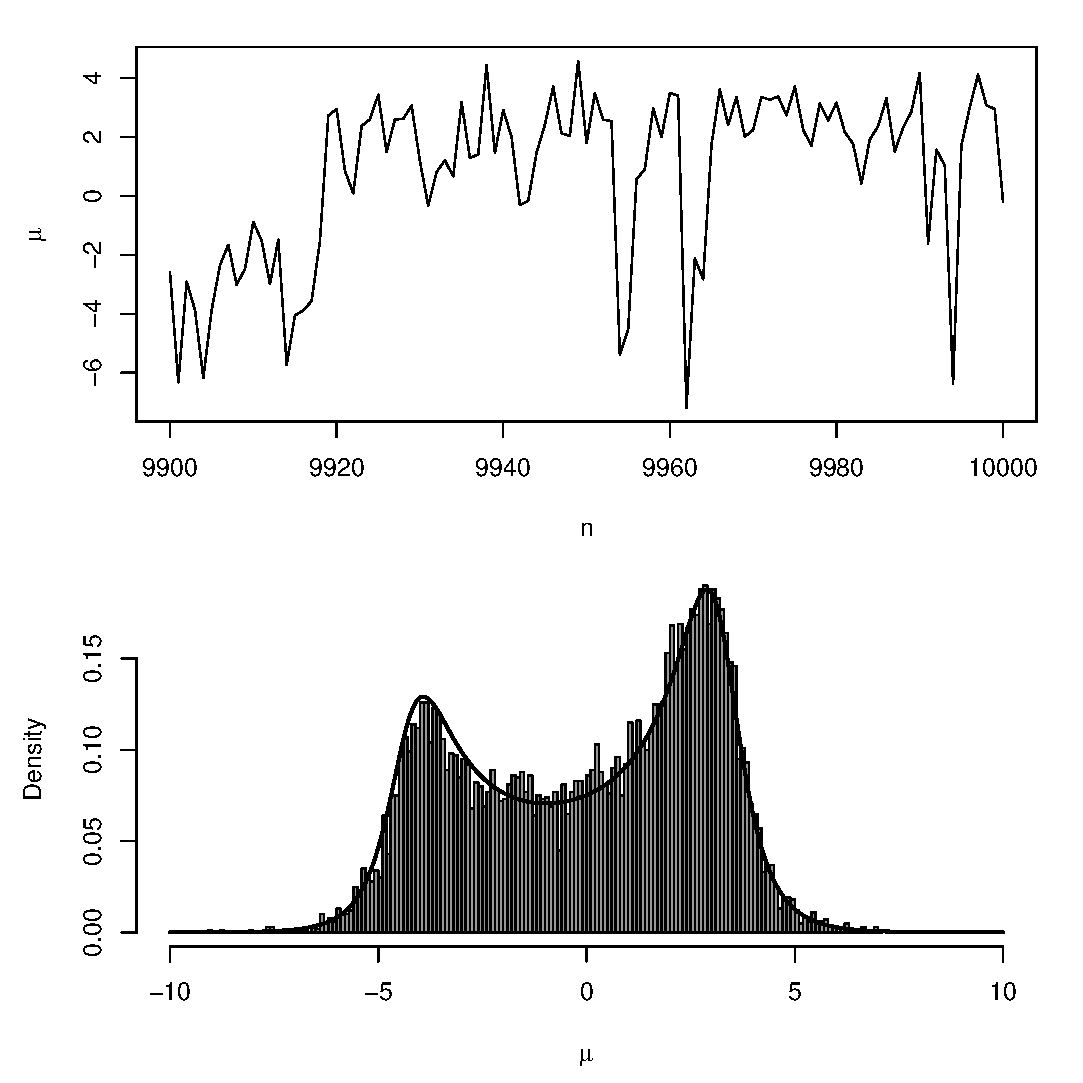
\includegraphics[width=7.5cm]{figures/simplegibbs.eps}}

\end{slide}\begin{slide}
\slidetitle{Generalisation}

Consider several groups of parameters, 
$\theta,\lambda_1,\allowbreak\ldots,\lambda_p$, such that
\[
\pi(\theta|x) = \int\ldots\int \pi(\theta,\lambda_1,\ldots,\lambda_p|x)
   \,d\lambda_1 \cdots \,d\lambda_p
\]
or simply divide $\theta$ in 
$$
(\theta_1,\ldots,\theta_p)
$$

\end{slide}\begin{slide}
\slidetitle{The general Gibbs sampler}

For a joint distribution $\pi(\theta)$ with full conditionals
$\pi_1,\ldots,\pi_p$,

\colorbox{LightGrey}{\makebox[0.9\textwidth][c]{\parbox{0.85\textwidth}{
{\sf
Given $(\theta_1^{(t)},\ldots,\theta_p^{(t)})$, simulate
\begin{itemize}
%\renewcommand{\theenumi}{\arabic{enumi}.}

\item[1.]  $\theta_1^{(t+1)} \sim
\pi_1(\theta_1|\theta_2^{(t)},\ldots,\theta_p^{(t)})$,

\item[2.] $\theta_2^{(t+1)} \sim
\pi_2(\theta_2|\theta_1^{(t+1)},\theta_3^{(t)},\ldots,\theta_p^{(t)})$,

\item[{\ }] $\qquad\qquad\vdots$

\item[p.] $\theta_p^{(t+1)} \sim
\pi_p(\theta_p|\theta_1^{(t+1)},\ldots,\theta_{p-1}^{(t+1)})$.
\end{itemize}
}}}}

\bigskip
\centerline{{{\bf Then $\theta^{(t)} \rightarrow \theta \sim \pi $}}}

\end{slide}
\normalsize \subsection{Variable selection}
\begin{slide}\slidetitle{Variable selection}

Back to regression: one dependent random variable $y$ and a set 
$\{x_1,\ldots,x_k\}$ of $k$ explanatory variables.

\pause
\vs\BrickRed{{\bf Question: }} Are all $x_i$'s involved in the regression?

\pause
\vs {\bf Assumption}: every subset $\{i_1,\ldots,i_q\}$ of 
$q$ $(0\le q\le k)$ explanatory variables, $\{\mathbf{1}_n,x_{i_1},
\ldots,x_{i_q}\}$, is a proper set of explanatory variables for the regression of $y$
[intercept included in every corresponding model] 

\pause
\begin{block}{Computational issue} 
\centerline{$2^k$ models in competition...}
\end{block}

\end{slide}\begin{slide}\slidetitle{Model notations}

\begin{enumerate}
\item $$
X=\left[\begin{matrix}\mathbf{1}_n &x_1 &\cdots &x_k \end{matrix}\right]
$$
is the matrix containing $\mathbf{1}_n$ and all the $k$ potential predictor variables

\item Each model $\mathfrak{M}_\gamma$ associated with binary indicator vector 
$\gamma\in\Gamma=\{0,1\}^k$ where $\gamma_i=1$ means that the variable $x_i$ is included in 
the model $\mathfrak{M}_\gamma$

\item $q_\gamma = \mathbf{1}_n^\tee \gamma$ number of variables included in the model $\mathfrak{M}_\gamma$

\item $t_1(\gamma)$ and $t_0(\gamma)$ indices of 
variables included in the model and indices of variables not included in the model
\end{enumerate}

\end{slide}\begin{slide}\slidetitle{Model indicators}

For $\beta\in\mathbb{R}^{k+1}$ and $X$, 
we define $\beta_\gamma$ as the subvector
$$
\beta_{\gamma}=\left(\beta_0,\left(\beta_i\right)_{i\in t_1(\gamma)}\right)
$$ 
and $X_{\gamma}$ as the submatrix of $X$ where only the column $\mathbf{1}_n$ 
and the columns in $t_1(\gamma)$ have been left.

\end{slide}\begin{slide}\slidetitle{Models in competition}

The model $\mathfrak{M}_\gamma$ is thus defined as 
$$
y|\gamma,\beta_\gamma,\sigma^2,X\sim\mathscr{N}_n\left(X_{\gamma}\beta_{\gamma},\sigma^2I_n\right)
$$
where $\beta_{\gamma}\in\mathbb{R}^{q_\gamma+1}$ and $\sigma^2\in\mathbb{R}^*_+$ 
are the unknown 
parameters.

\pause\vs
\begin{block}{Warning}
$\sigma^2$ is common to all models and thus uses the same prior for all models
\end{block}

\end{slide}\begin{slide}\slidetitle{Informative $G$-prior}

Many ($2^k$) models in competition: we cannot expect 
a practitioner to specify a prior on every $\mathfrak{M}_\gamma$ 
in a completely subjective and autonomous manner. 

\vs \BurntOrange{{\bf Shortcut:}} We derive {\em all} priors from a single 
global prior associated with the so-called {\em full model} that corresponds 
to $\gamma=(1,\dots,1)$. 

\end{slide}\begin{slide}\slidetitle{Prior definitions}

\begin{enumerate}
\renewcommand{\theenumi}{(\roman{enumi})}
\item For the full model, Zellner's $G$-prior:
$$
\beta|\sigma^2,X\sim\mathscr{N}_{k+1}(\tilde\beta,c\sigma^2(X^\tee X)^{-1})
\quad\text{and}\quad
\sigma^2\sim \pi(\sigma^2|X)=\sigma^{-2}
$$
\item For each model $\mathfrak{M}_\gamma$, the prior distribution of $\beta_{\gamma}$ 
conditional on $\sigma^2$ is fixed as
$$
\beta_\gamma|\gamma,\sigma^2 \sim \mathcal{N}_{q_\gamma+1}\left(\tilde\beta_{\gamma},
	c\sigma^2\left(X_{\gamma}^\tee X_{\gamma}\right)^{-1}\right)\,,
$$
where $\tilde \beta_\gamma=\left(X_\gamma^TX_\gamma\right)^{-1}X_\gamma^T\tilde\beta$
and same prior on $\sigma^2$. 
\end{enumerate}

\end{slide}\begin{slide}\slidetitle{Prior completion}

The joint prior for model $\mathfrak{M}_\gamma$ is
the improper prior
\begin{eqnarray*}
\pi(\beta_\gamma,\sigma^2|\gamma) 
&\propto& \left(\sigma^2\right)^{-(q_\gamma+1)/2-1}
   \exp\left[-\frac{1}{2(c\sigma^2)}\left(\beta_{\gamma}-\tilde\beta_{\gamma}\right)^\tee \right.\\
&&\quad \left.(X_{\gamma}^\tee X_{\gamma})\left(\beta_{\gamma}-\tilde\beta_{\gamma}\right)\right]\,.
\end{eqnarray*}

\end{slide}\begin{slide}\slidetitle{Prior competition (2)}

Infinitely many ways of defining a prior on the model index 
$\gamma$: choice of uniform prior $\pi(\gamma|X)=2^{-k}$.

\vs Posterior distribution of $\gamma$ central to 
variable selection since it is proportional to marginal density of $y$ on 
$\mathfrak{M}_\gamma$ (or {\em evidence} of $\mathfrak{M}_\gamma$)
\small
\begin{eqnarray*}
\pi(\gamma|y,X) & \propto & f(y|\gamma,X)\pi(\gamma|X) \propto f(y|\gamma,X) \\
                & = & \int\left(\int f(y|\gamma,\beta,\sigma^2,X)\pi(\beta|\gamma,
			\sigma^2,X)\,\text{d}\beta\right)\pi(\sigma^2|X)\,\text{d}\sigma^2\,.
\end{eqnarray*}
\normalsize

\end{slide}\begin{slide}
\small \begin{eqnarray*}
f(y|\gamma,\sigma^2,X) &=& \int f(y|\gamma,\beta,\sigma^2)\pi(\beta|\gamma,\sigma^2)\,\text{d}\beta \\
                       &=& (c+1)^{-(q_\gamma+1)/2}(2\pi)^{-n/2}\left(\sigma^2\right)^{-n/2} 
				\,\exp\left(-\frac{1}{2\sigma^2}y^\tee y \right.\\
                       & &\ \left.+\frac{1}{2\sigma^2(c+1)}\left\{c y^\tee X_{\gamma}\left(X_{\gamma}^\tee 
			     X_{\gamma}\right)^{-1}X_{\gamma}^\tee y
                       -\tilde\beta_{\gamma}^\tee X_{\gamma}^\tee X_{\gamma} \tilde\beta_{\gamma}\right\}\right)\,,
\end{eqnarray*}
\normalsize
this posterior density satisfies
\begin{eqnarray*}
\pi(\gamma|y,X) &\propto& (c+1)^{-(q_\gamma+1)/2}\left[y^\tee y-\frac{c}{c+1}y^\tee X_{\gamma}\left(X_{\gamma}^\tee 
			X_{\gamma}\right)^{-1}X_{\gamma}^\tee y\right. \\
                &&\quad \left.-\frac{1}{c+1}\tilde\beta_{\gamma}^\tee X_{\gamma}^\tee X_{\gamma} \tilde\beta_{\gamma}\right]^{-n/2}.
\end{eqnarray*}
\normalsize

\end{slide}\begin{frame} \frametitle{Pine processionary caterpillars} 

\begin{center}
\footnotesize
\begin{tabular}{l c| r}
  $t_1(\gamma)\ $ && $\ \pi(\gamma|\by,X)$ \\
 \hline 0,1,2,4,5 && 0.2316 \\
 0,1,2,4,5,9   && 0.0374 \\
 0,1,9         && 0.0344 \\
 0,1,2,4,5,10  && 0.0328 \\
 0,1,4,5       && 0.0306 \\
 0,1,2,9       && 0.0250 \\
 0,1,2,4,5,7   && 0.0241 \\
 0,1,2,4,5,8   && 0.0238 \\
 0,1,2,4,5,6   && 0.0237 \\
 0,1,2,3,4,5   && 0.0232 \\
 0,1,6,9       && 0.0146 \\
 0,1,2,3,9     && 0.0145 \\
 0,9           && 0.0143 \\
 0,1,2,6,9     && 0.0135 \\
 0,1,4,5,9     && 0.0128 \\
 0,1,3,9       && 0.0117 \\
 0,1,2,8       && 0.0115 \\
\end{tabular}                      
\normalsize
\end{center}

\end{frame}\begin{frame} \frametitle{Pine processionary caterpillars (cont'd)}

\begin{block}{Interpretation} Model $\mathfrak{M}_\gamma$ with the highest posterior probability
is $t_1(\gamma)=(1,2,4,5)$, which corresponds to the variables
\begin{itemize}
\item[-] altitude,
\item[-] slope,
\item[-] height of the tree sampled in the center of the area, and
\item[-] diameter of the tree sampled in the center of the area.
\end{itemize}
\end{block}

\pause\vs
Corresponds to the five variables identified in the {\sf R} regression output

\end{frame}\begin{slide}
\slidetitle{Noninformative extension}

For Zellner noninformative prior with $\pi(c)=1/c$, we have
\begin{eqnarray*}
\pi(\gamma|y,X)&\propto&\sum_{c=1}^\infty c^{-1}(c+1)^{-(q_\gamma+1)/2}\left[y^\tee y-\right.\nonumber\\
&&\quad \left.\frac{c}{c+1}y^\tee X_{\gamma}\left(X_{\gamma}^\tee X_{\gamma}\right)^{-1}X_{\gamma}^\tee y\right]^{-n/2}.
\end{eqnarray*}

\end{slide}\begin{frame} \frametitle{Pine processionary caterpillars}

\begin{center}
\footnotesize
\begin{tabular}{l c|r}
 $t_1(\gamma)$ && $\ \pi(\gamma|\by,X)$ \\ 
\hline 
 0,1,2,4,5      && 0.0929 \\
 0,1,2,4,5,9    && 0.0325 \\
 0,1,2,4,5,10   && 0.0295 \\
 0,1,2,4,5,7    && 0.0231 \\
 0,1,2,4,5,8    && 0.0228 \\
 0,1,2,4,5,6    && 0.0228 \\
 0,1,2,3,4,5    && 0.0224 \\
 0,1,2,3,4,5,9  && 0.0167 \\
 0,1,2,4,5,6,9  && 0.0167 \\
 0,1,2,4,5,8,9  && 0.0137 \\
 0,1,4,5        && 0.0110 \\
 0,1,2,4,5,9,10 && 0.0100 \\
 0,1,2,3,9      && 0.0097 \\
 0,1,2,9        && 0.0093 \\
 0,1,2,4,5,7,9  && 0.0092 \\
 0,1,2,6,9      && 0.0092 \\
\end{tabular}
\normalsize
\end{center}

\end{frame}\begin{slide}
\slidetitle{Stochastic search for the most likely model}

When $k$ gets large, impossible to compute the 
posterior probabilities of the $2^k$ models. 

\pause\vs
Need of a tailored algorithm 
that samples from $\pi(\gamma|y,X)$ and 
selects the most likely models. 

\vs Can be done by Gibbs sampling, given the availability 
of the full conditional posterior probabilities of the $\gamma_i$'s.

If $\gamma_{-i}=(\gamma_1,\ldots,\gamma_{i-1},\gamma_{i+1},\ldots,\gamma_k)$ 
($1\le i\le k$) 
$$
\pi(\gamma_i|y,\gamma_{-i},X)\propto
\pi(\gamma|y,X)
$$
(to be evaluated in both $\gamma_i=0$ and $\gamma_i=1$)

\end{slide}\begin{slide}\slidetitle{Gibbs sampling for variable selection}

\colorbox{LightGrey}{\makebox[0.9\textwidth][c]{\parbox{0.85\textwidth}{
\begin{sffamily}
\begin{itemize}
\item[ ] {\bfseries Initialization:} Draw $\gamma^0$ from the uniform distribution on $\Gamma$
\pause\vspace{0.5cm} \item[ ] {\bfseries Iteration $t$:} Given $(\gamma_1^{(t-1)},\ldots,\gamma_k^{(t-1)})$, generate
\begin{itemize}
\vspace{0.25cm} \item[1.] {{ \ $\gamma_1^{(t)}$ according to 
$\pi(\gamma_1|y,\gamma_2^{(t-1)},\ldots,\gamma_k^{(t-1)},X)$ }}
\vspace{0.25cm} \item[2.] {{ \ $\gamma_2^{(t)}$ according to 
$\pi(\gamma_2|y,\gamma_1^{(t)},\gamma_3^{(t-1)},\ldots,\gamma_k^{(t-1)},X)$ }}
\vspace{0.25cm} \item[{\ }] $\qquad\qquad\vdots$
\vspace{0.25cm} \item[p.] {{ \ $\gamma_k^{(t)}$ according to 
$\pi(\gamma_k|y,\gamma_1^{(t)},\ldots,\gamma_{k-1}^{(t)},X)$ }}
\end{itemize}
\end{itemize}
\end{sffamily}
}}}

\end{slide}\begin{slide}\slidetitle{MCMC interpretation}

After $T\gg 1$ MCMC iterations,
output used to approximate the posterior probabilities $\pi(\gamma|y,X)$ 
by empirical averages 
$$
\widehat{\pi}(\gamma|y,X)=\left(\frac{1}{T-T_0+1}\right)\sum_{t=T_0}^T \mathbb{I}_{\gamma^{(t)}=\gamma}.
$$
where the $T_0$ first values are eliminated as {\em burnin}.

\pause\vs
And approximation of the probability to include $i$-th variable,
$$
{\widehat{P}}^\pi(\gamma_i=1|y,X)=\left(\frac{1}{T-T_0+1}\right)\sum_{t=T_0}^T 
\mathbb{I}_{\gamma^{(t)}_i=1}\,.
$$
\end{slide}\begin{slide}\slidetitle{Pine processionary caterpillars}

\begin{center}
\small
\begin{tabular}{l c|r|r}
 $\gamma_i$    && $\ {\widehat{P}}^\pi(\gamma_i=1|\by,X)$ 
& $\ {\widehat{P}}^\pi (\gamma_i=1|\by,X)$\\                                                    
\hline $\gamma_1$    && 0.8624 & 0.8844 \\
 $\gamma_2$    && 0.7060 & 0.7716 \\
 $\gamma_3$    && 0.1482 & 0.2978 \\
 $\gamma_4$    && 0.6671 & 0.7261 \\
 $\gamma_5$    && 0.6515 & 0.7006 \\
 $\gamma_6$    && 0.1678 & 0.3115 \\
 $\gamma_7$    && 0.1371 & 0.2880 \\
 $\gamma_8$    && 0.1555 & 0.2876 \\
 $\gamma_9$    && 0.4039 & 0.5168 \\
 $\gamma_{10}$ && 0.1151 & 0.2609 \\
\end{tabular}
\normalsize

Probabilities of inclusion with both informative
$(\tilde\beta=0_{11},c=100)$ and noninformative  Zellner's priors 
\end{center}


\end{slide}
